% Chapter Template

\chapter{Outros tópicos de ML} % Main chapter title

\label{ChapterX} % Change X to a consecutive number; for referencing this chapter elsewhere, use \ref{ChapterX}

%----------------------------------------------------------------------------------------
%	SECTION 1
%----------------------------------------------------------------------------------------

\section{“Off-the-Shelf” Procedures for Data Mining}
Predictive learning is an important aspect of data mining. As can be seen
from this book, a wide variety of methods have been developed for predic-
tive learning from data. For each particular method there are situations
for which it is particularly well suited, and others where it performs badly
compared to the best that can be done with that data. We have attempted
to characterize appropriate situations in our discussions of each of the re-
spective methods. However, it is seldom known in advance which procedure
will perform best or even well for any given problem. Table 10.1 summarizes
some of the characteristics of a number of learning methods.
Industrial and commercial data mining applications tend to be especially
challenging in terms of the requirements placed on learning procedures.
Data sets are often very large in terms of number of observations and
number of variables measured on each of them. Thus, computational considerations play an important role. Also, the data are usually messy: the
inputs tend to be mixtures of quantitative, binary, and categorical vari-
ables, the latter often with many levels. There are generally many missing
values, complete observations being rare. Distributions of numeric predic-
tor and response variables are often long-tailed and highly skewed. This
is the case for the spam data (Section 9.1.2); when fitting a generalized
additive model, we first log-transformed each of the predictors in order to
get a reasonable fit. In addition they usually contain a substantial fraction
of gross mis-measurements (outliers). The predictor variables are generally
measured on very different scales.
In data mining applications, usually only a small fraction of the large
number of predictor variables that have been included in the analysis are
actually relevant to prediction. Also, unlike many applications such as pat-
tern recognition, there is seldom reliable domain knowledge to help create
especially relevant features and/or filter out the irrelevant ones, the inclu-
sion of which dramatically degrades the performance of many methods.
In addition, data mining applications generally require interpretable mod-
els. It is not enough to simply produce predictions. It is also desirable to
have information providing qualitative understanding of the relationship
between joint values of the input variables and the resulting predicted re-
sponse value. Thus, black box methods such as neural networks, which can
be quite useful in purely predictive settings such as pattern recognition,
are far less useful for data mining.
These requirements of speed, interpretability and the messy nature of
the data sharply limit the usefulness of most learning procedures as off-
the-shelf methods for data mining. An “off-the-shelf” method is one that
can be directly applied to the data without requiring a great deal of time-
consuming data preprocessing or careful tuning of the learning procedure.
Of all the well-known learning methods, decision trees come closest to
meeting the requirements for serving as an off-the-shelf procedure for data
mining. They are relatively fast to construct and they produce interpretable
models (if the trees are small). As discussed in Section 9.2, they naturally
incorporate mixtures of numeric and categorical predictor variables and
missing values. They are invariant under (strictly monotone) transforma-
tions of the individual predictors. As a result, scaling and/or more general
transformations are not an issue, and they are immune to the effects of pre-
dictor outliers. They perform internal feature selection as an integral part
of the procedure. They are thereby resistant, if not completely immune,
to the inclusion of many irrelevant predictor variables. These properties of
decision trees are largely the reason that they have emerged as the most
popular learning method for data mining.
Trees have one aspect that prevents them from being the ideal tool for
predictive learning, namely inaccuracy. They seldom provide predictive ac-
curacy comparable to the best that can be achieved with the data at hand.
As seen in Section 10.1, boosting decision trees improves their accuracy,
often dramatically. At the same time it maintains most of their desirable
properties for data mining. Some advantages of trees that are sacrificed by
boosting are speed, interpretability, and, for AdaBoost, robustness against
overlapping class distributions and especially mislabeling of the training
data. A gradient boosted model (GBM) is a generalization of tree boosting
that attempts to mitigate these problems, so as to produce an accurate and
effective off-the-shelf procedure for data mining.

\begin{figure}[H]
\centering
\caption{LearningMethods}
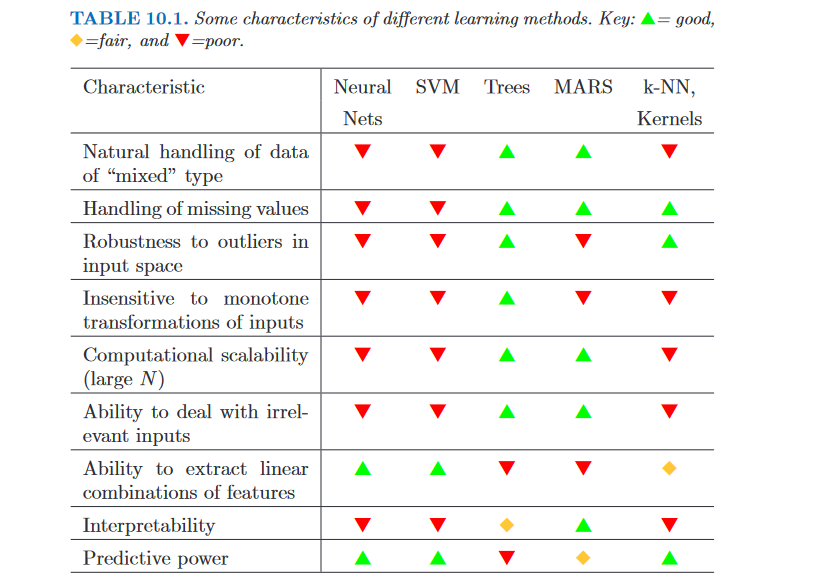
\includegraphics[scale=.7]{Figures/learning-methods.PNG}
\end{figure}

\section{Principal Components Analysis}
The basic goal of principal components analysis is to describe variation in a set of correlated variables, $\textbf{x}^T = (x_1, \dots, x_q)$ in terms of new set of uncorrelated variables $\textbf{y}^T = (y_1, \dots, y_q)$, each of which is a linear combination of the $\textbf{x}$ variables.

The new variables are derived in decreasing order of “impor-
tance” in the sense that $y_1$ accounts for as much as possible of the variation in
the original data amongst all linear combinations of $\textbf{x}$. Then $y_2$ is chosen to
account for as much as possible of the remaining variation, subject to being
uncorrelated with $y_1$, and so on. The new variables defined by this process,
$y_1, \dots, y_q$ , are the principal components.

The first principal component of the observations, y1, is the linear combination

\begin{equation}
    y_1 = a_{11}x_1 + a_{12}x_2 + \dots + a_{1q}x_q
\end{equation}

whose sample variance is greatest among all such linear combinations. Because the variance of $y_1$ could be increased without limit simply by increasing the coefficients $a_1^T = (a_{11}, a_{12}, \dots, a_{1q}x_q)$, a restriction must be placed on these coefficients. To find the coefficients defining the first principal component, we need to choose the elements of the vector  $\textbf{a}_1$
so as to maximize the variance of $y_1$ subject to the sum of squares constraint, which can be written $\textbf{a}_1^T\textbf{a}_1 = 1$. The sample variance of $y_1$ that is a linear function of the $x$ variables is given by $\textbf{a}_1^T\textbf{S}\textbf{a}_1 = 1$, where $S$ is the $q x q$ sample covariance matrix of the $x$ variables. Lagrange multiplier approach leads to the solution that $\textbf{a}_1$ is the eigenvector of the sample covariance matrix, $\textbf{S}$, corresponding to this matrix's largest eigenvalue. The eigenvalues $\lambda$ and eigenvectors $\gamma$ of a $q x q$ matrix $\textbf{A}$ are such that $\textbf{A}\gamma = \lambda\gamma$.

The second principal component, y2, is defined to be the linear combination

\begin{equation}
    y_2 = a_{21}x_1 + a_{22}x_2 + \dots + a_{2q}x_q
\end{equation}

(i.e, $y_2 = \textbf{a}_2^T$\textbf{x}, $a_2^T = (a_{21}, a_{22}, \dots, a_{2q}x_q)$ and $\textbf{x}^T = (x_1, \dots, x_q)$) that has the greatest variance subject to the following conditions:

\begin{equation}
    \textbf{a}_2^T\textbf{a}_2 = 1 (normalized)
\end{equation}

\begin{equation}
    \textbf{a}_2^T\textbf{a}_1 = 0 (orthogonal)
\end{equation}

(The second condition ensures that $y_1$ and $y_2$ are uncorrelated.

Application of the Lagrange multiplier technique demonstrates that the vector
of coefficients defining the jth principal component, $\textbf{a}_j$ , is the eigenvector of $\textbf{S}$ associated with its jth largest eigenvalue.


\section{Missing data}
Missing data can be MAR, MCAR, and MNAR.

\begin{itemize}
    \item MCAR (Missing completely at random): The values in the missing column are randomly missing and do not depend on the other column values.
    \item MAR (Missing at random): The values in the missing column are dependent on some additional features.
    \item MNAR (Missing not at random): The data is not missing randomly there might be some reason behind that.
    
    Lembrar do exemplo do Vincent Warmerdam: uma pessoa registra as alturas das pessoas que aparecem com a cabela acima do muro de sua casa. Os dados serão viesados pois as pessoas com altura abaixo do muro não serão utlizadas!!!
\end{itemize}

\section{Data imputation}

\begin{itemize}
    \item Imputation using (mean/median) values
    \item Imputation using (most frequent) or (Zero/Constant) values
    \item Imputation using k-NN
    \item Imputation using Multivariate Imputation by Chained Equation (MICE)
    \item Stochastic regression imputation: similar to regression imputation which tries to predict the missing values by regressing it from other related variables in the same dataset plus some random residual value
\end{itemize}

\section{Como lidar com evento raro?}
\begin{itemize}
    \item \textbf{Oversampling}: simple to implement and fast to execute, which is desirable for very large and complex datasets
    \item \textbf{Undersampling:} simple to implement and fast to execute, which is desirable for very large and complex datasets
    \item \textbf{SMOTE (Synthetic Minority Oversampling Technique)}: Specifically, a random example from the minority class is first chosen. Then k of the nearest neighbors for that example are found (typically k=5). A randomly selected neighbor is chosen and a synthetic example is created at a randomly selected point between the two examples in feature space. It is vital that you do not use SMOTE on the full data set. You MUST use SMOTE on the training set only (after you split). Then validate on your val/test sets and see if your SMOTE model out performed your other model(s). If you do not do this there will be data leakage and your model is essentially cheating.
\end{itemize}

\section{Feature Selection}
\subsection{Permutation Importance}
No contexto de redes neurais ou black-box models, como funciona o algoritmo:

\begin{enumerate}
\item Ajusta-se o modelo e calcula-se a métrica de avaliação.
\item Para cada covariável, será feito uma permutação na ordem da covariável.
\item Então calcula-se novamente a métrica de avaliação para o modelo com a covariável permutada.
\item Então, compara-se a métrica original com a métrica da variável permutada. Essa variação da métrica original será considerada como a importância da covariável permutada. Obs.: Pode-se repetir o passo 4 várias vezes, tomando a média do processo como a importância da variável.
\end{enumerate}

\subsection{Computing the amount of Impurity}
Computing the amount of Impurity (typically variance in case of regression trees and gini coefficient or entropy in case of classification trees) each feature removes when it is used in node.

\subsection{Boruta}
No contexto de random forests for regression, Boruta is a feature selection algorithm which is statistically grounded and works extremely well even without any specific input by the user.
    
\begin{enumerate}
\item In practice, starting from X, another dataframe is created by randomly shuffling each feature. These permuted features are called \textbf{shadow features}. At this point, the shadow dataframe is attached to the original dataframe to obtain a new dataframe (we will call it X\_boruta), which has twice the number of columns of X.

Now, we take the importance of each original features and compare it with a threshold. This time, the threshold is defined as the highest feature importance recorded among the shadow features. When the importance of a feature is higher than this threshold, this is called a “hit”. The idea is that a feature is useful only if it is capable of doing better than the best randomized feature.

\item The maximum level of uncertainty about the feature is expressed by a probability of 50\%, like tossing a coin. Since each independent experiment can give a binary outcome (hit or no hit), a series of n trials follows a binomial distribution.
\end{enumerate}

\section{Tipos de Amostragem}

\subsection{Amostragem sistemática}
Utilizada quando os elementos estão dispostos de maneira organizada (ex.: fila, lista) e aleatória. Escolhe um ponto de partida e seleciona-se cada k -ésimo elemento da população (ex.: o 50◦elemento). Por exemplo, Em uma fábrica de lâmpadas, a cada 100 peças produzidas, uma é retirada para teste.

\subsection{Amostragem Estratificada}
Indicada quando a população está dividida em grupos distintos, denominados estratos. Dentro de cada estrato é realizada uma amostragem aleatória simples. O tamanho da amostra pode ou não ser proporcional ao tamanho do estrato. Por exemplo, uma comunidade universitária com 8000 indivíduos está estratificada da seguinte forma Estrato = [Professores, Funcionários, Estudantes], População = [800, 1200, 6000] e Amostra = [80, 120, 600]
    
\subsection{Amostragem por Conglomerado}
A área da população é dividida em seções (ou conglomerados, ex.: bairros, quarteirões). Os conglomerados são selecionados aleatoriamente. Dentro de um conglomerado, todos os elementos são amostrados.


\subsection{Calibration}
Adjusting the predictions of a model so that they are probabilistically meaningful.
